\chapter{Legoblokdetectie op meerdere niveau's}
\label{hoofdstuk:4}
Na het vorige hoofdstuk beseffen we dat legoblokconstructies van meerdere niveau's moeilijk kunnen worden gedetecteerd door alle legoblokken individueel te detecteren. Bovendien zijn we op zoek naar een algoritme waarvan de performantie haalbaar wordt voor een AR spel. Daarom wordt in dit hoofdstuk geopperd om de legoblokconstructie te detecteren alvorens het spel wordt gespeeld. De scheiding van deze twee fases zorgt ervoor dat we minder beperkt zijn in de performantie van de legoblokdetectie, dit mag immers meerdere frames duren omdat ervan wordt uitgegaan dat de constructie niet meer veranderd. Het algoritme baseert zich op het na\"ieve detectie-algoritme van hoofdstuk \ref{hoofdstuk:2} maar gaat op een meer intelligente manier om met de informatie die uit de contouren kan worden gehaald.


\section{Begrippen}

\section{Algoritme}
Het algoritme verloopt in drie fasen die in deze sectie worden besproken: calibratie, detectie van de legowereld en het spel. De calibratiefase zorgt ervoor dat we  minder afhankelijk zijn van de belichting waarin het detectie-algoritme wordt uitgevoerd. In feite worden de kleuren van de legoblokken opgemeten en gebruikt om te bepalen welke waarden voor de kleurthreshold moeten worden gebruikt. 

\subsection{Calibratie}
\begin{figure}
  \centering
	\begin{tikzpicture}
	    \node[anchor=south west,inner sep=0] (image) at (0,0) {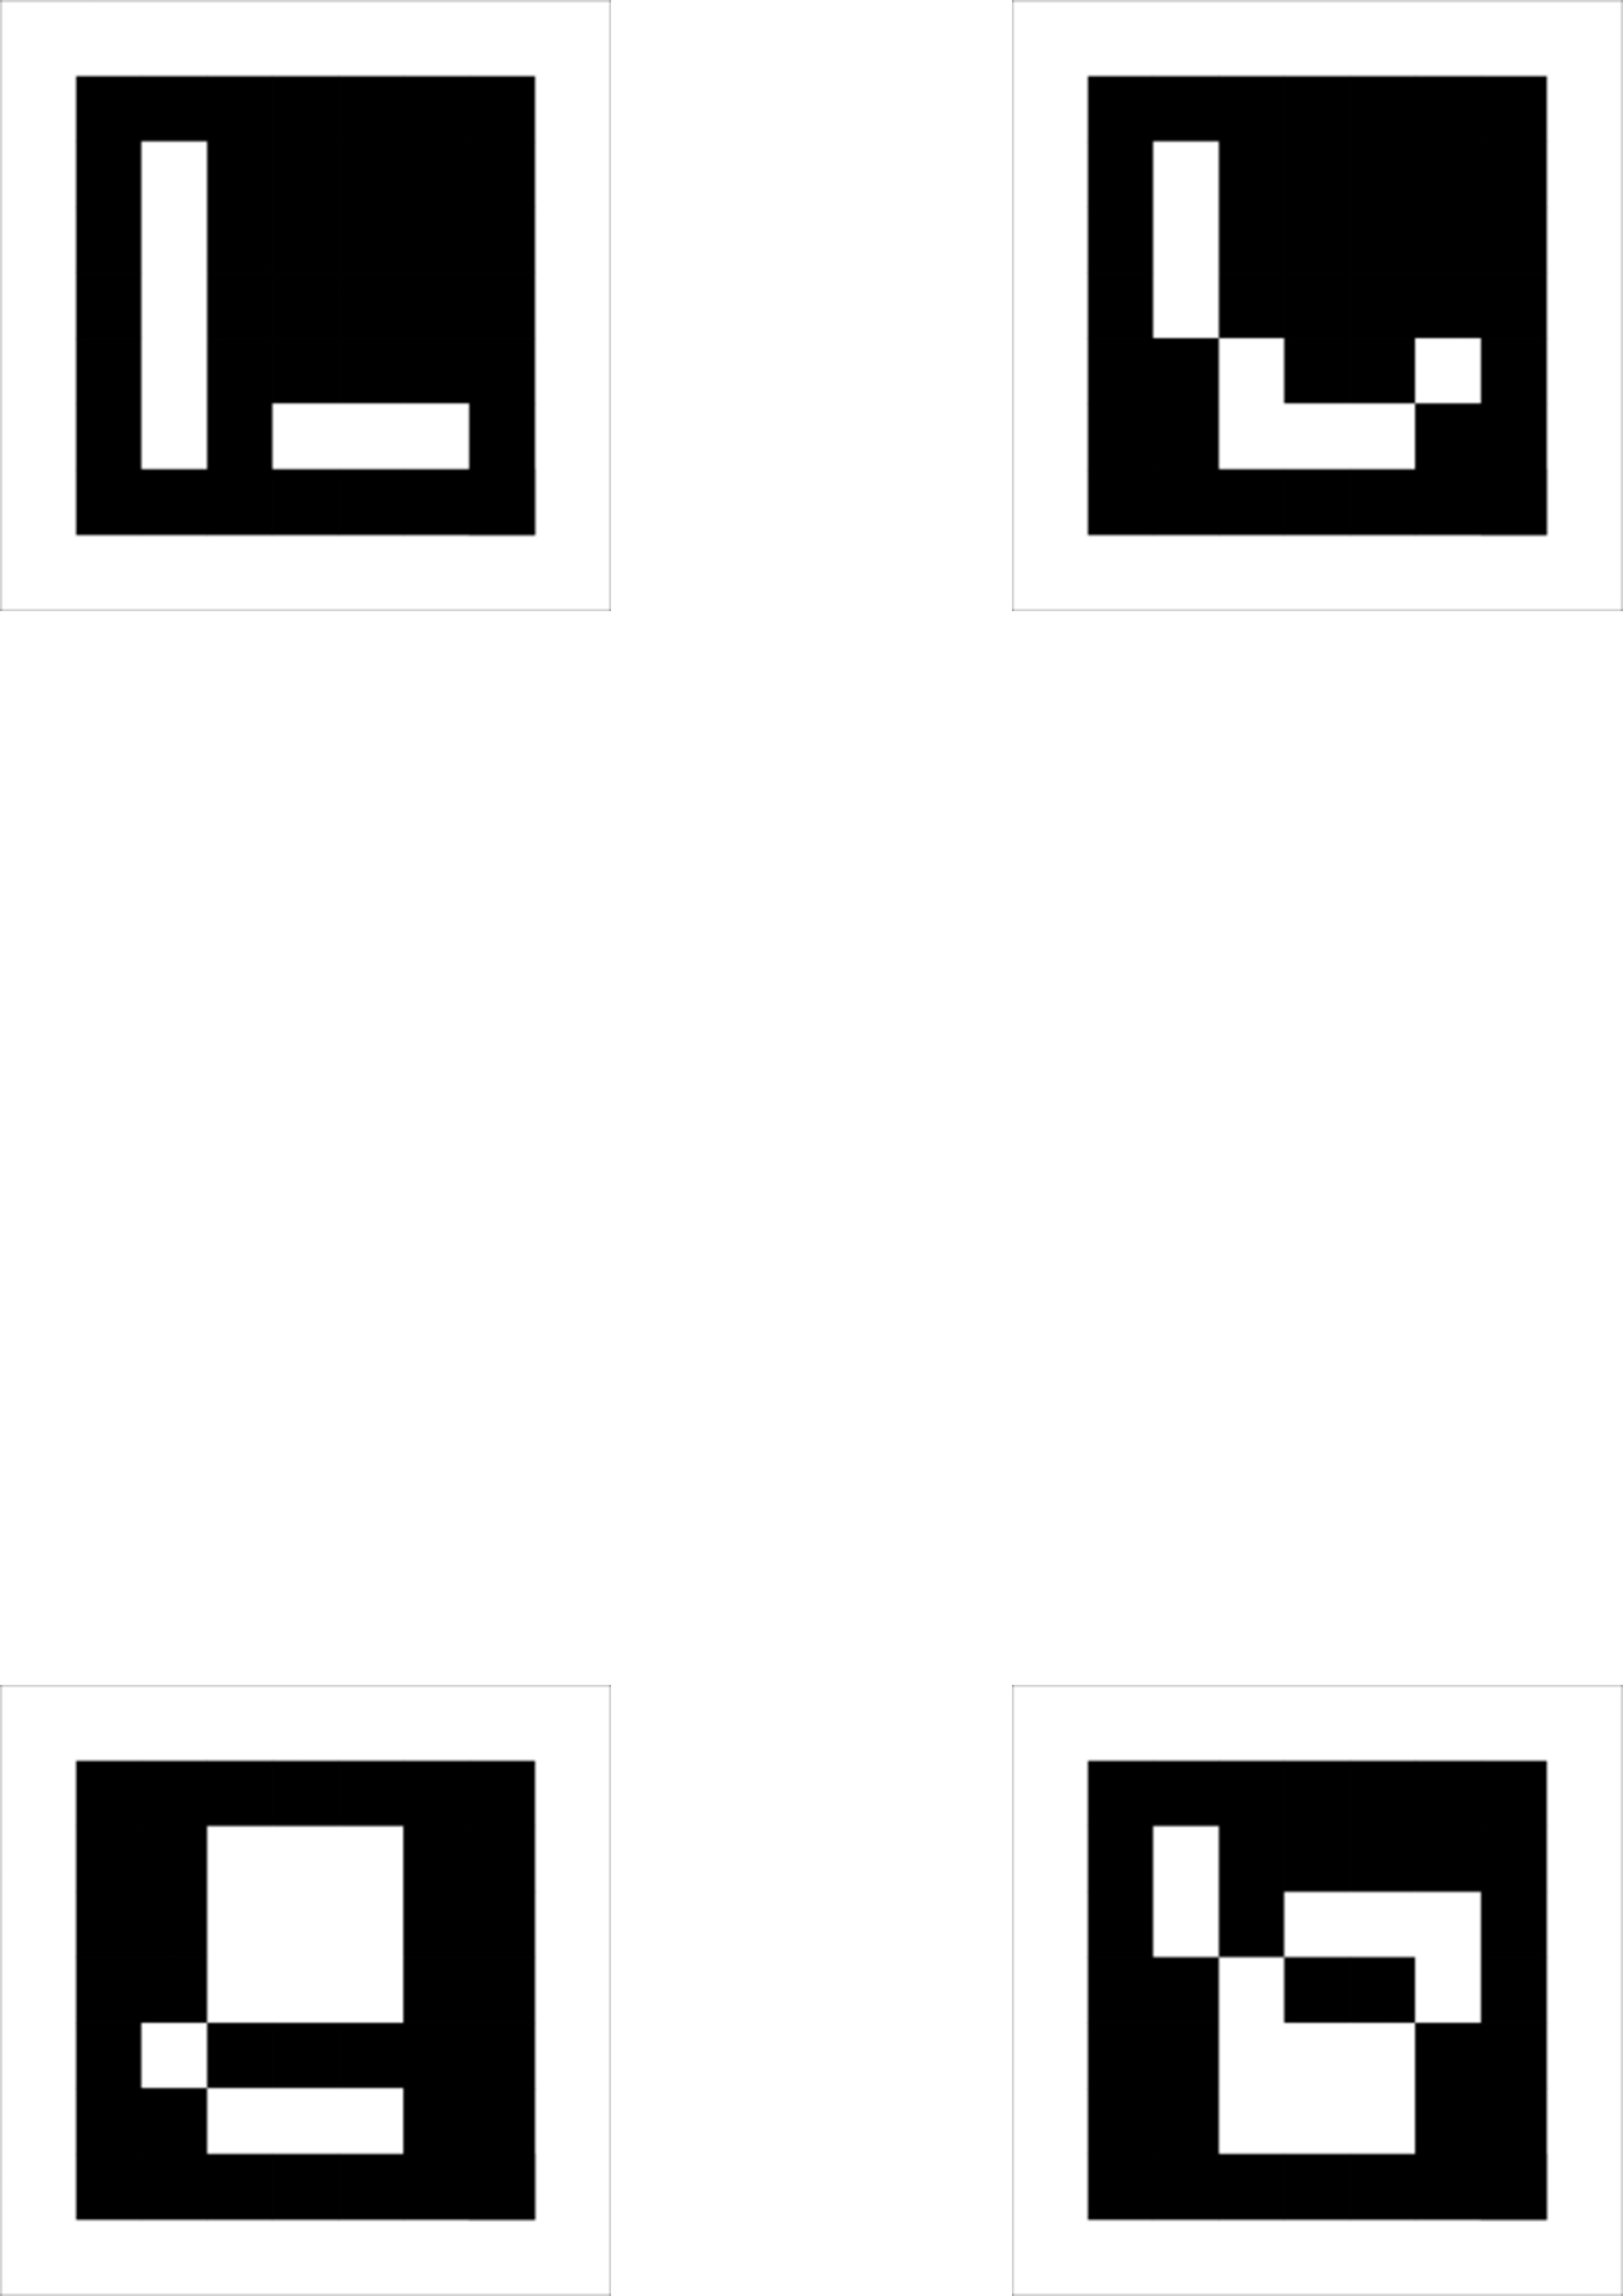
\includegraphics[width=0.5\textwidth]{img/armarkers}};
	    \begin{scope}[x={(image.south east)},y={(image.north west)}]
	        \draw[red,ultra thick,rounded corners,<->] (0.10,-0.05) node[red,below]{2} to [bend left=45] (-0.05,0.10) node[red,left]{1};
	        \draw[ultra thick] (0.5,-0.10) -- (0.45,-0.05);
	        \draw[ultra thick] (0.5,-0.10) -- (0.55,-0.05);
	        \draw (0.47,-0.06) to [bend left=45] (0.53,-0.06);
%	       \filldraw[fill=white, draw=black] (0.5,-0.065) ellipse (0.015 and 0.0106);
	       \filldraw[fill=black, draw=black] (0.5,-0.055) ellipse (0.02 and 0.0048);
	        \filldraw[fill=red, draw=black] (0.83,0.6735) rectangle (1,0.7335);
	        \filldraw[fill=yellow, draw=black] (0.83,0.2665) rectangle (1,0.3265);
	    \end{scope}
	\end{tikzpicture}
	\caption{Deze figuur toont hoe de calibratiefase met twee kleuren verloopt.}
	\label{fig:calib}
\end{figure}

Deze fase is erg belangrijk om te bepalen in welke belichting we de legoblokken willen gaan detecteren. Het idee is dat de speler per gebruikte kleur een 2x4 legoblok van 2 hoog op een specifieke plaats op het grondvlak plaatst. Vervolgens draait de speler het grondvlak langzaam een kwartslag heen en terug. Figuur \ref{fig:calib} toont een grafische weergave van dit proces. Het rode en gele vlak zijn twee legoblokjes van verschillende kleur, het oog onderaan is de camera en de rode pijl geeft aan in welke richting het grondvlak wordt gedraaid, dus eerst met de klok mee en vervolgens in tegenwijzerzin. 

\section{Tweede onderwerp in dit hoofdstuk}

\section{Besluit}

%%% Local Variables: 
%%% mode: latex
%%% TeX-master: "masterproef"
%%% End: 
